

\tikzset{every picture/.style={line width=0.75pt}} %set default line width to 0.75pt        

\begin{tikzpicture}[x=0.75pt,y=0.75pt,yscale=-1,xscale=1]
%uncomment if require: \path (0,287); %set diagram left start at 0, and has height of 287

%Image [id:dp6789989035032795] 
\draw (331.45,190.67) node  {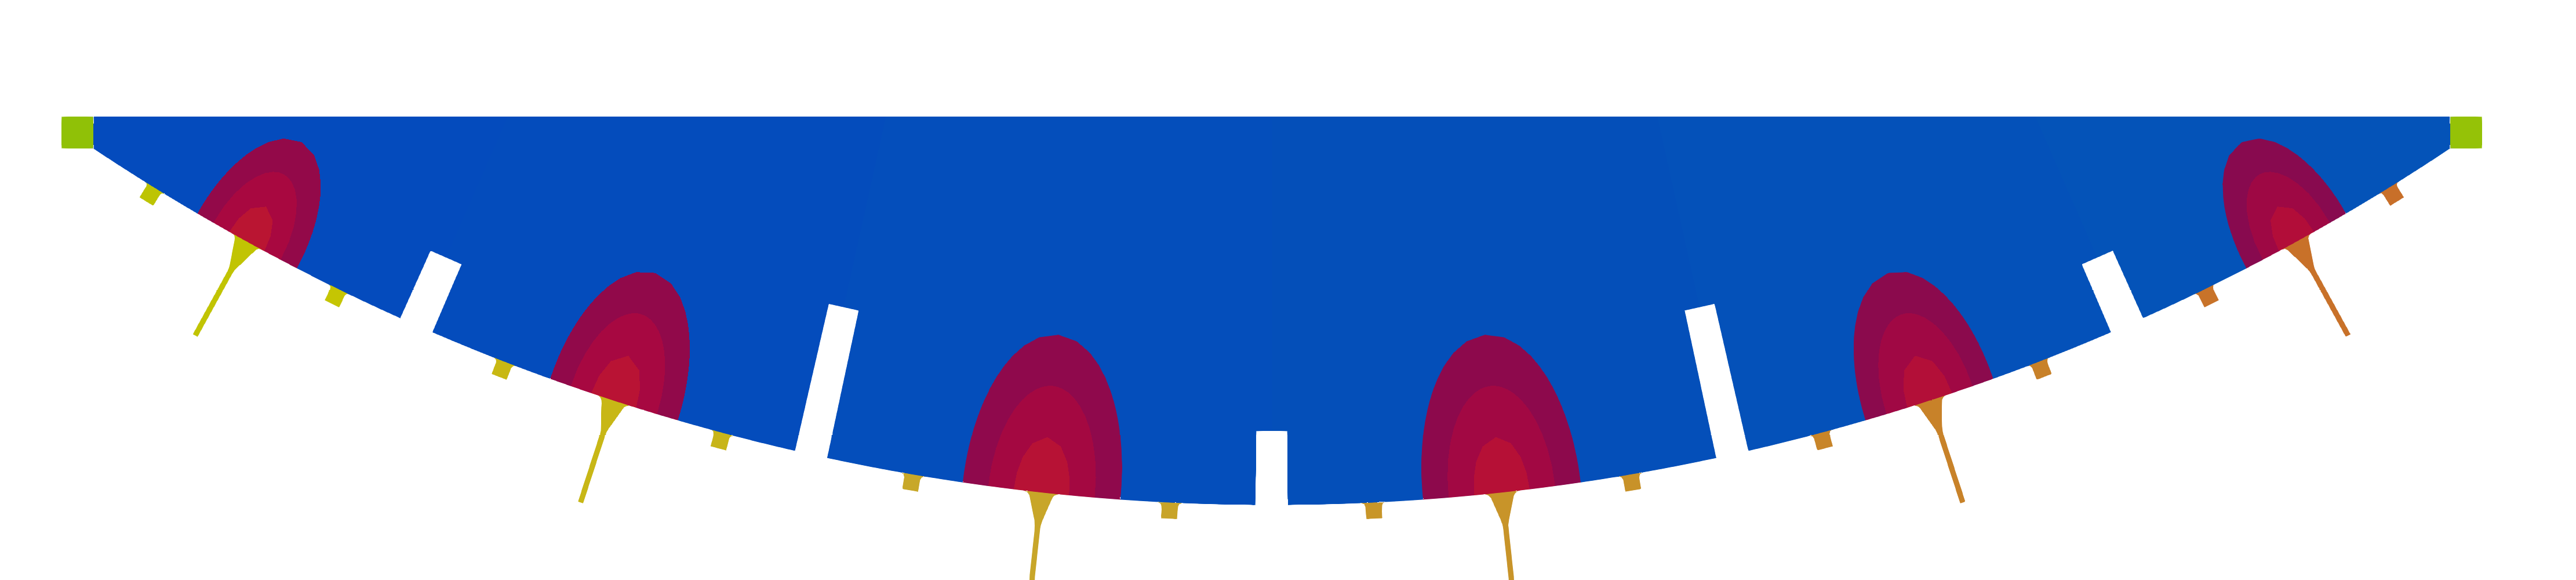
\includegraphics[width=482.17pt,height=108.5pt]{diagrams/placenta-geometry-diagrams/region_inverted-circle-slice-6-flat_normal-walls.png}};
%Shape: Polygon [id:ds5403154356225157] 
\draw  [fill={rgb, 255:red, 155; green, 155; blue, 155 }  ,fill opacity=0.2 ] (472.82,276.51) -- (410.33,270) -- (410.33,197.67) -- (472.82,13.58) -- cycle ;
%Shape: Rectangle [id:dp4374039436651571] 
\draw   (359.25,197.67) -- (410.33,197.67) -- (410.33,270) -- (359.25,270) -- cycle ;
%Shape: Rectangle [id:dp8847560919034154] 
\draw   (19.67,140.67) -- (37.17,140.67) -- (37.17,158.42) -- (19.67,158.42) -- cycle ;
%Shape: Rectangle [id:dp5761346961280844] 
\draw   (230.08,231.83) -- (247.58,231.83) -- (247.58,247.33) -- (230.08,247.33) -- cycle ;
%Shape: Polygon [id:ds6386627939021934] 
\draw  [fill={rgb, 255:red, 155; green, 155; blue, 155 }  ,fill opacity=0.2 ] (171.58,112.75) -- (37.17,140.67) -- (19.67,140.67) -- (15.25,112.75) -- cycle ;
%Shape: Polygon [id:ds9675166776770578] 
\draw  [fill={rgb, 255:red, 155; green, 155; blue, 155 }  ,fill opacity=0.2 ] (384.08,130) -- (247.58,231.83) -- (230.08,231.83) -- (259.58,130) -- cycle ;
%Shape: Rectangle [id:dp40877732662413346] 
\draw  [color={rgb, 255:red, 74; green, 144; blue, 226 }  ,draw opacity=1 ][fill={rgb, 255:red, 255; green, 255; blue, 255 }  ,fill opacity=1 ][line width=2.25] [blur shadow={shadow xshift=0pt,shadow yshift=0pt, shadow blur radius=1.5pt, shadow blur steps=4 ,shadow opacity=100}] (259.58,27.8) -- (384.08,27.8) -- (384.08,130) -- (259.58,130) -- cycle ;
%Shape: Rectangle [id:dp3581407575862343] 
\draw  [color={rgb, 255:red, 74; green, 144; blue, 226 }  ,draw opacity=1 ][fill={rgb, 255:red, 255; green, 255; blue, 255 }  ,fill opacity=1 ][line width=2.25] [blur shadow={shadow xshift=0pt,shadow yshift=0pt, shadow blur radius=1.5pt, shadow blur steps=4 ,shadow opacity=100}] (15.25,19.67) -- (171.58,19.67) -- (171.58,112.75) -- (15.25,112.75) -- cycle ;
%Image [id:dp5821978380209227] 
\draw (106.1,65.26) node  {
\includegraphics[width=75.15pt,height=61.39pt]{diagrams/placenta-geometry-diagrams/region_inverted-circle-slice-6-flat_normal-walls_marginal-sinus.png}};
%Straight Lines [id:da3775297991043933] 
\draw [color={rgb, 255:red, 74; green, 144; blue, 226 }  ,draw opacity=1 ][line width=3.75]    (330.25,101.5) -- (302,97.25) ;
%Straight Lines [id:da9001565707068373] 
\draw [color={rgb, 255:red, 74; green, 144; blue, 226 }  ,draw opacity=1 ][line width=3.75]    (65.25,79.75) -- (65.25,34.25) ;
%Shape: Axis 2D [id:dp5537933186782882] 
\draw  (10.68,267.79) -- (43.48,267.79)(13.96,238.27) -- (13.96,271.07) (36.48,262.79) -- (43.48,267.79) -- (36.48,272.79) (8.96,245.27) -- (13.96,238.27) -- (18.96,245.27)  ;

%Shape: Rectangle [id:dp6146437218873158] 
\draw  [color={rgb, 255:red, 208; green, 2; blue, 27 }  ,draw opacity=1 ][fill={rgb, 255:red, 255; green, 255; blue, 255 }  ,fill opacity=1 ][line width=2.25] [blur shadow={shadow xshift=0pt,shadow yshift=0pt, shadow blur radius=1.5pt, shadow blur steps=4 ,shadow opacity=100}] (472.82,13.58) -- (645.15,13.58) -- (645.15,276.51) -- (472.82,276.51) -- cycle ;
%Image [id:dp8106950500710235] 
\draw (560.93,139.16) node  {
\includegraphics[width=117.17pt,height=171.38pt]{diagrams/placenta-geometry-diagrams/region_inverted-circle-slice-6-flat_normal-walls_artery.png}};
%Shape: Arc [id:dp897401775896993] 
\draw  [draw opacity=0][line width=3.75]  (518.97,160.96) .. controls (518.96,160.86) and (518.95,160.76) .. (518.94,160.66) .. controls (514.6,115.21) and (529.36,76.62) .. (551.91,74.46) .. controls (574.31,72.32) and (595.97,106.92) .. (600.53,151.92) -- (559.78,156.76) -- cycle ; \draw  [line width=3.75]  (518.97,160.96) .. controls (518.96,160.86) and (518.95,160.76) .. (518.94,160.66) .. controls (514.6,115.21) and (529.36,76.62) .. (551.91,74.46) .. controls (574.31,72.32) and (595.97,106.92) .. (600.53,151.92) ;  
%Straight Lines [id:da8094844692675482] 
\draw    (526.82,210.91) -- (556.86,194.36) ;
\draw [shift={(559.48,192.91)}, rotate = 151.14] [fill={rgb, 255:red, 0; green, 0; blue, 0 }  ][line width=0.08]  [draw opacity=0] (8.93,-4.29) -- (0,0) -- (8.93,4.29) -- cycle    ;
%Straight Lines [id:da3729402376326847] 
\draw [color={rgb, 255:red, 208; green, 2; blue, 27 }  ,draw opacity=1 ][line width=2.25]    (571.15,241.16) -- (567.15,241.66) ;
%Straight Lines [id:da14537836403413262] 
\draw [color={rgb, 255:red, 155; green, 155; blue, 155 }  ,draw opacity=1 ] [dash pattern={on 0.84pt off 2.51pt}]  (583.37,175.64) -- (581.15,154.91) ;
%Straight Lines [id:da6003461463769395] 
\draw [color={rgb, 255:red, 155; green, 155; blue, 155 }  ,draw opacity=1 ] [dash pattern={on 0.84pt off 2.51pt}]  (602.13,164.6) -- (600.53,151.92) ;
%Image [id:dp29326967503664414] 
\draw (320.41,80.83) node  {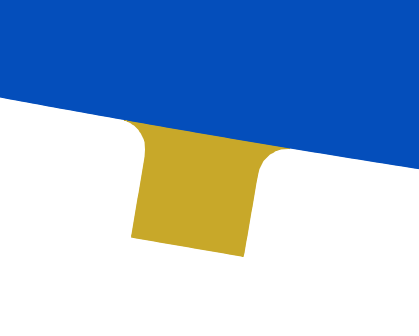
\includegraphics[width=79.62pt,height=63.85pt]{diagrams/placenta-geometry-diagrams/region_inverted-circle-slice-6-flat_normal-walls_vein.png}};
%Straight Lines [id:da9436862634001915] 
\draw [color={rgb, 255:red, 178; green, 15; blue, 57 }  ,draw opacity=1 ]   (566.73,177.64) -- (580.39,176) ;
\draw [shift={(583.37,175.64)}, rotate = 173.14] [fill={rgb, 255:red, 178; green, 15; blue, 57 }  ,fill opacity=1 ][line width=0.08]  [draw opacity=0] (5.36,-2.57) -- (0,0) -- (5.36,2.57) -- cycle    ;
\draw [shift={(563.75,178)}, rotate = 353.14] [fill={rgb, 255:red, 178; green, 15; blue, 57 }  ,fill opacity=1 ][line width=0.08]  [draw opacity=0] (5.36,-2.57) -- (0,0) -- (5.36,2.57) -- cycle    ;
%Straight Lines [id:da9114914997274575] 
\draw [color={rgb, 255:red, 178; green, 15; blue, 57 }  ,draw opacity=1 ]   (564.98,169.14) -- (599.15,164.96) ;
\draw [shift={(602.13,164.6)}, rotate = 173.03] [fill={rgb, 255:red, 178; green, 15; blue, 57 }  ,fill opacity=1 ][line width=0.08]  [draw opacity=0] (5.36,-2.57) -- (0,0) -- (5.36,2.57) -- cycle    ;
\draw [shift={(562,169.5)}, rotate = 353.03] [fill={rgb, 255:red, 178; green, 15; blue, 57 }  ,fill opacity=1 ][line width=0.08]  [draw opacity=0] (5.36,-2.57) -- (0,0) -- (5.36,2.57) -- cycle    ;
%Straight Lines [id:da8852053594450542] 
\draw [color={rgb, 255:red, 178; green, 15; blue, 57 }  ,draw opacity=1 ]   (564.48,160.39) -- (619.02,153.86) ;
\draw [shift={(622,153.5)}, rotate = 173.17] [fill={rgb, 255:red, 178; green, 15; blue, 57 }  ,fill opacity=1 ][line width=0.08]  [draw opacity=0] (5.36,-2.57) -- (0,0) -- (5.36,2.57) -- cycle    ;
\draw [shift={(561.5,160.75)}, rotate = 353.17] [fill={rgb, 255:red, 178; green, 15; blue, 57 }  ,fill opacity=1 ][line width=0.08]  [draw opacity=0] (5.36,-2.57) -- (0,0) -- (5.36,2.57) -- cycle    ;
%Straight Lines [id:da9553990232091423] 
\draw [color={rgb, 255:red, 74; green, 144; blue, 226 }  ,draw opacity=1 ][line width=3.75]    (329.25,103) -- (300.5,97.5) ;
%Straight Lines [id:da9713029290513338] 
\draw    (353.4,105.62) -- (336.4,95.9) ;
\draw [shift={(333.8,94.42)}, rotate = 29.74] [fill={rgb, 255:red, 0; green, 0; blue, 0 }  ][line width=0.08]  [draw opacity=0] (7.14,-3.43) -- (0,0) -- (7.14,3.43) -- cycle    ;
%Straight Lines [id:da5454083808690029] 
\draw [color={rgb, 255:red, 0; green, 0; blue, 0 }  ,draw opacity=1 ] [dash pattern={on 0.84pt off 2.51pt}]  (339.25,89.52) -- (303.5,82.27) ;
%Straight Lines [id:da8936020822292747] 
\draw [color={rgb, 255:red, 178; green, 15; blue, 57 }  ,draw opacity=1 ]   (341.4,78.94) -- (339.85,86.58) ;
\draw [shift={(339.25,89.52)}, rotate = 281.5] [fill={rgb, 255:red, 178; green, 15; blue, 57 }  ,fill opacity=1 ][line width=0.08]  [draw opacity=0] (3.57,-1.72) -- (0,0) -- (3.57,1.72) -- cycle    ;
\draw [shift={(342,76)}, rotate = 101.5] [fill={rgb, 255:red, 178; green, 15; blue, 57 }  ,fill opacity=1 ][line width=0.08]  [draw opacity=0] (3.57,-1.72) -- (0,0) -- (3.57,1.72) -- cycle    ;
%Straight Lines [id:da49992139569120564] 
\draw [color={rgb, 255:red, 0; green, 0; blue, 0 }  ,draw opacity=1 ] [dash pattern={on 0.84pt off 2.51pt}]  (91.6,77.97) -- (91.91,44.01) -- (92,33.57) ;
%Straight Lines [id:da35794129578966505] 
\draw    (55,93.02) -- (71.76,82.51) ;
\draw [shift={(74.3,80.92)}, rotate = 147.91] [fill={rgb, 255:red, 0; green, 0; blue, 0 }  ][line width=0.08]  [draw opacity=0] (7.14,-3.43) -- (0,0) -- (7.14,3.43) -- cycle    ;
%Straight Lines [id:da44499881038098454] 
\draw [color={rgb, 255:red, 178; green, 15; blue, 57 }  ,draw opacity=1 ]   (94.5,82.8) -- (108,82.98) ;
\draw [shift={(111,83.02)}, rotate = 180.73] [fill={rgb, 255:red, 178; green, 15; blue, 57 }  ,fill opacity=1 ][line width=0.08]  [draw opacity=0] (5.36,-2.57) -- (0,0) -- (5.36,2.57) -- cycle    ;
\draw [shift={(91.5,82.77)}, rotate = 0.73] [fill={rgb, 255:red, 178; green, 15; blue, 57 }  ,fill opacity=1 ][line width=0.08]  [draw opacity=0] (5.36,-2.57) -- (0,0) -- (5.36,2.57) -- cycle    ;
%Straight Lines [id:da602787461013311] 
\draw [color={rgb, 255:red, 128; green, 128; blue, 128 }  ,draw opacity=1 ] [dash pattern={on 0.84pt off 2.51pt}]  (98.15,77.87) -- (98.55,33.47) ;
%Straight Lines [id:da9481149805723406] 
\draw [color={rgb, 255:red, 128; green, 128; blue, 128 }  ,draw opacity=1 ] [dash pattern={on 0.84pt off 2.51pt}]  (104.65,77.87) -- (105.05,33.47) ;
%Straight Lines [id:da30724585431443985] 
\draw [color={rgb, 255:red, 128; green, 128; blue, 128 }  ,draw opacity=1 ] [dash pattern={on 0.84pt off 2.51pt}]  (332.25,83.02) -- (304.25,77.52) ;
%Straight Lines [id:da9604038006149647] 
\draw [color={rgb, 255:red, 128; green, 128; blue, 128 }  ,draw opacity=1 ] [dash pattern={on 0.84pt off 2.51pt}]  (333.25,78.02) -- (303.75,72.52) ;

% Text Node
\draw (326.38,181.58) node  [font=\LARGE,color={rgb, 255:red, 255; green, 255; blue, 255 }  ,opacity=1 ]  {$\Omega _{\text{IVS}}$};
% Text Node
\draw (355.09,102.52) node [anchor=north west][inner sep=0.75pt]  [font=\small,color={rgb, 255:red, 0; green, 0; blue, 0 }  ,opacity=1 ]  {$\Omega _{\text{v}}$};
% Text Node
\draw (337.04,55.71) node  [font=\LARGE,color={rgb, 255:red, 255; green, 255; blue, 255 }  ,opacity=1 ]  {$\Omega _{\text{IVS}}$};
% Text Node
\draw (56.84,82.4) node [anchor=north east] [inner sep=0.75pt]  [font=\Large,color={rgb, 255:red, 0; green, 0; blue, 0 }  ,opacity=1 ]  {$\Omega _{\text{v}}$};
% Text Node
\draw (133.71,58.91) node  [font=\normalsize,color={rgb, 255:red, 255; green, 255; blue, 255 }  ,opacity=1 ]  {$\Omega _{\text{IVS}}$};
% Text Node
\draw (316.29,105.22) node [anchor=north] [inner sep=0.75pt]  [font=\small,color={rgb, 255:red, 74; green, 144; blue, 226 }  ,opacity=1 ]  {$\Gamma _{\text{out}}$};
% Text Node
\draw (59.86,58.16) node [anchor=east] [inner sep=0.75pt]  [font=\large,color={rgb, 255:red, 74; green, 144; blue, 226 }  ,opacity=1 ]  {$\Gamma _{\text{out}}$};
% Text Node
\draw (46.86,264.31) node [anchor=west] [inner sep=0.75pt]  [font=\footnotesize]  {$x$};
% Text Node
\draw (15,231.86) node [anchor=south] [inner sep=0.75pt]  [font=\footnotesize]  {$y$};
% Text Node
\draw (558.69,142.08) node  [font=\normalsize,color={rgb, 255:red, 255; green, 255; blue, 255 }  ,opacity=1 ]  {$\Omega _{\text{CC}}$};
% Text Node
\draw (612.44,46.16) node  [font=\large,color={rgb, 255:red, 255; green, 255; blue, 255 }  ,opacity=1 ]  {$\Omega _{\text{IVS}}$};
% Text Node
\draw (524.82,214.31) node [anchor=north east] [inner sep=0.75pt]  [font=\LARGE,color={rgb, 255:red, 0; green, 0; blue, 0 }  ,opacity=1 ]  {$\Omega _{\text{a}}$};
% Text Node
\draw (572.4,245.56) node [anchor=north] [inner sep=0.75pt]  [font=\Large,color={rgb, 255:red, 208; green, 2; blue, 27 }  ,opacity=1 ]  {$\Gamma _{\text{in}}$};
% Text Node
\draw (574.99,179.12) node [anchor=north] [inner sep=0.75pt]  [font=\normalsize,color={rgb, 255:red, 0; green, 0; blue, 0 }  ,opacity=1 ,rotate=-353.1]  {$\textcolor[rgb]{0.64,0.04,0.26}{r}\textcolor[rgb]{0.64,0.04,0.26}{_{0}}$};
% Text Node
\draw (594.74,168.12) node [anchor=north] [inner sep=0.75pt]  [font=\normalsize,color={rgb, 255:red, 0; green, 0; blue, 0 }  ,opacity=1 ,rotate=-353.1]  {$\textcolor[rgb]{0.64,0.04,0.26}{r}\textcolor[rgb]{0.64,0.04,0.26}{_{1}}$};
% Text Node
\draw (612.99,157.62) node [anchor=north] [inner sep=0.75pt]  [font=\normalsize,color={rgb, 255:red, 0; green, 0; blue, 0 }  ,opacity=1 ,rotate=-353.1]  {$\textcolor[rgb]{0.64,0.04,0.26}{r}\textcolor[rgb]{0.64,0.04,0.26}{_{2}}$};
% Text Node
\draw (555.94,99.83) node  [font=\normalsize,color={rgb, 255:red, 255; green, 255; blue, 255 }  ,opacity=1 ]  {$\Omega {_{\text{T}^{-}}^{\ }}^{\ }$};
% Text Node
\draw (553.19,54.08) node  [font=\normalsize,color={rgb, 255:red, 255; green, 255; blue, 255 }  ,opacity=1 ]  {$\Omega {_{\text{T}^{+}}^{\ }}^{\ }$};
% Text Node
\draw (344.31,82.55) node [anchor=west] [inner sep=0.75pt]  [font=\scriptsize,color={rgb, 255:red, 0; green, 0; blue, 0 }  ,opacity=1 ,rotate=-9.23]  {$\textcolor[rgb]{0.64,0.04,0.26}{y}\textcolor[rgb]{0.64,0.04,0.26}{_{0}}$};
% Text Node
\draw (101.81,85.16) node [anchor=north] [inner sep=0.75pt]  [font=\scriptsize,color={rgb, 255:red, 0; green, 0; blue, 0 }  ,opacity=1 ]  {$\textcolor[rgb]{0.64,0.04,0.26}{y}\textcolor[rgb]{0.64,0.04,0.26}{_{0}}$};


\end{tikzpicture}
